 \author{Ricardo Krause}
\section{MotrXP GUI}

		\begin{frame}{MotrXP GUI}{Anforderungen}
		\textbf{Funktionale Anforderungen:}
	  		\begin{itemize}
	   	 		\item Anzeige der Sensordaten
	    		\item Regelung der Drehgeschwindigkeit
	    		\item Einstellung des PID Reglers
	  		\end{itemize}
	  		\textbf{Nicht-Funktionale Anforderungen:}
	  		\begin{itemize}
	   	 		\item Modulares erweiterbares System 
	    		\item Modernes Metro Design
	  		\end{itemize}
		\end{frame}

		\begin{frame}{MotrXP GUI}{Entwurf}
		\begin{minipage}{0.6\textwidth}
			\begin{itemize}
				\item Drei Schichten Architektur
	   	 		\item Entwurfsmuster
	    		\item DatenStrukturen
	    		\item Mockup
	  		\end{itemize}
		\end{minipage}
		\hfill
	  		\begin{minipage}{0.3\textwidth}
	  			\begin{figure}[htbp]
	  				\centering
	  				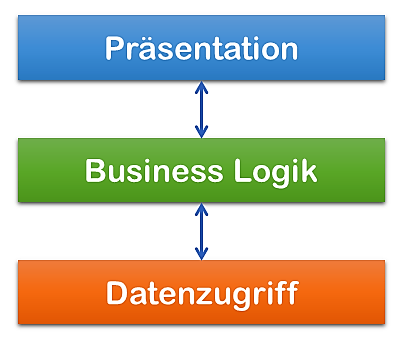
\includegraphics[width=\textwidth]{../gui/Bilder/Arc1.png}
	  			\end{figure}
	  			\begin{figure}[h]
	  				\centering
	  				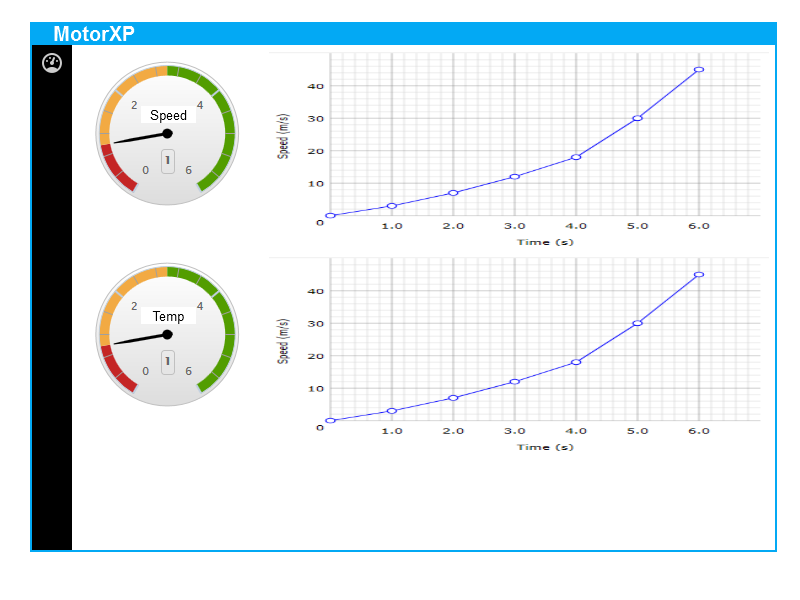
\includegraphics[width=\textwidth]{../gui/Bilder/Mockup.png}
	  			\end{figure}
	  		\end{minipage}
	  		
	  		
		\end{frame}

		\begin{frame}{MotrXP GUI}{Implementierung}
		\begin{minipage}{0.5\textwidth}
			\begin{itemize}
				\item MVVM-Light Framework
				\item MahApps Metro UI Toolkit
				\item Custom Controls 
			\end{itemize}
		\end{minipage}
		\hfill
		\begin{minipage}{0.4\textwidth}
			\begin{figure}[h]
	  			\centering
	  				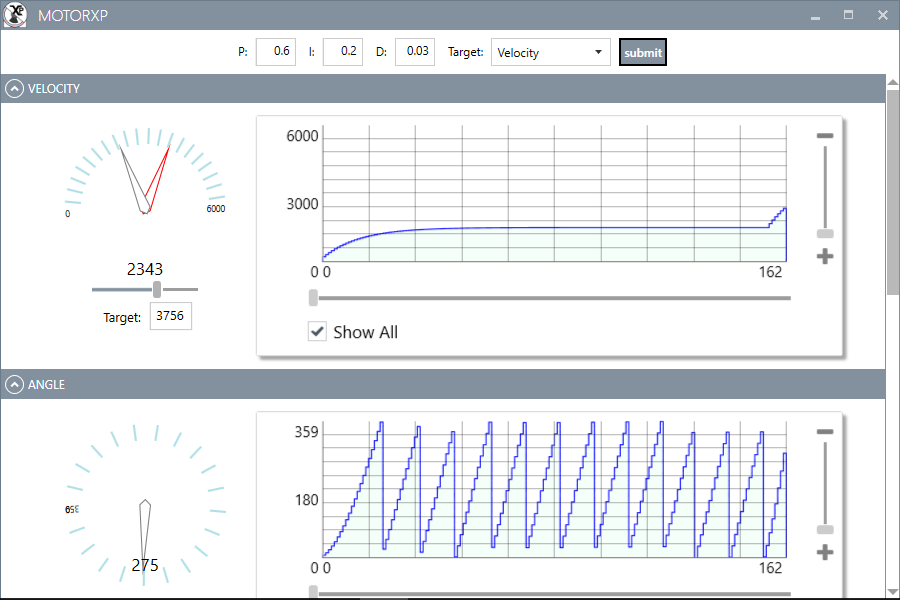
\includegraphics[width=\textwidth]{../gui/Bilder/GUIScreenshot2.png}
	  		\end{figure}
		\end{minipage}
	  		
		\end{frame}


		\begin{frame}{MotrXP GUI}{Ausblick}
\begin{figure}
	  			\centering
	  				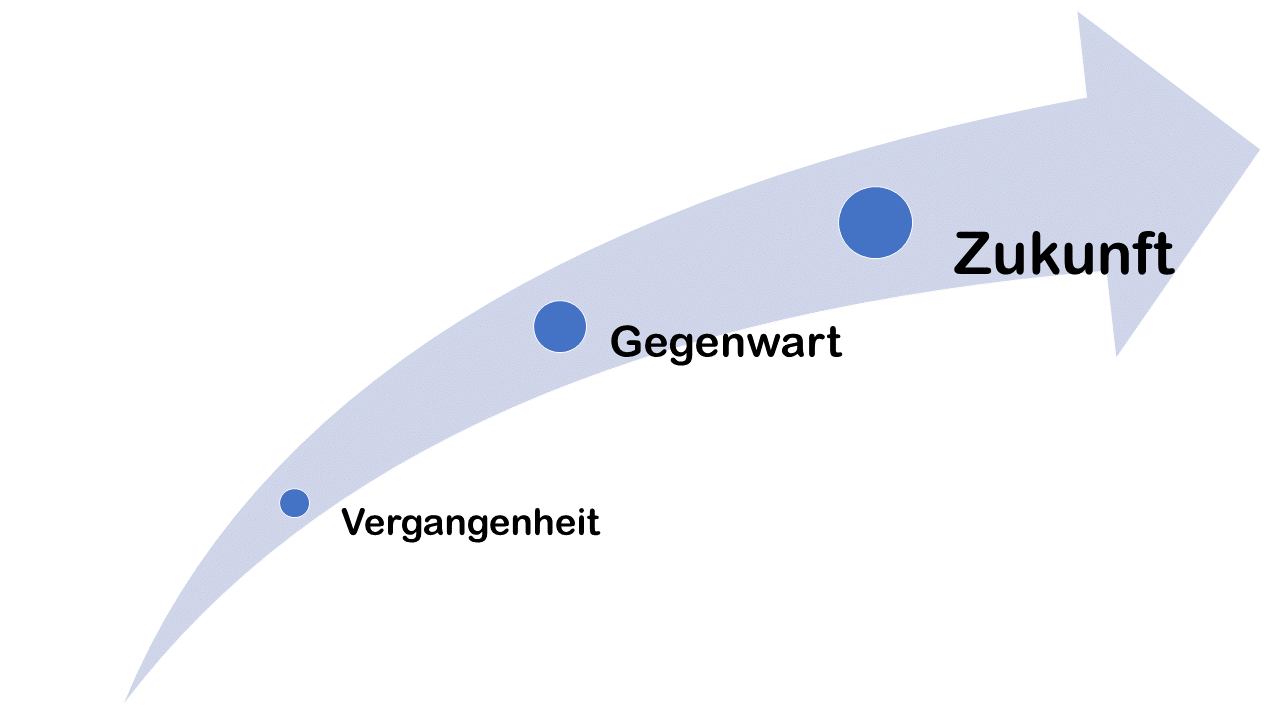
\includegraphics[width=\textwidth]{../gui/Bilder/AusblickPfeil.png}
	  		\end{figure}
		\end{frame}